\subsection{Replication}

\begin{itemize}
    \item
      Improve performance. How it does?
    \item
      Share workload in order to increase \emph{throughput} of served
      requests and reduce the \emph{latency} for individual requests
    \item
      Replicate data close to the users to reduce the \emph{latency} for
      individual requests (like CDN approach). This is true not only in DS
      but also in parallel systems
    \item
      Fault tolerance. How it does?
    \item
      Increase availability, because data may be available only
      intermittently in a mobile settings
    \item
      Achieve fault tolerance: related to availability data may become
      unavailable due to failure
\end{itemize}

\subsubsection{Consistency}

The main problem in \textbf{replication} is the \textbf{consistency}. In
particular changing a replica demands changes to all the other, but, if
we update multiple replicas concurrently we will have \emph{write-write}
and \emph{read-write} conflicts. It's important to notice that replication 
may actually degrade performance because of the overhead needed to make all 
this system works may have a bad influence.

Ideally, a read should show the result of the last write, but what does
\emph{last} mean? It's impossible to determine without a global clock.\\

\subsubsection{Some concept and definition}

\textbf{Consistency models}: a consistency model is a contract between
the processes and the data store.\\
\textbf{Guarantees on content}: set the maximum ``difference'' on the
versions stored at different replicas. \emph{For example, if I want some
macro statistics I can accept some difference, but not if I'm managing
my money.}\\
\textbf{Guarantees on staleness}: set the maximum time between a change
and its propagation to all replicas, in other words, I don't want data
older than a certain period. \emph{For example, for daily backups, it's
possible to lose data, but at least I have a checkpoint, that in this
case correspond to yesterday backup.}\\
\textbf{Guarantees on the order of updates}: constrain the possible
behaviors in the case of conflicts.

\subsection{Consistency protocols implement consistency model}

There are different strategies for different assumptions/configurations:

\subparagraph{Passive vs active}

\begin{itemize}
    \item
      \textbf{Passive}: there is only one machine that works on data.
      \emph{e.g.~the hard disk backup is a passive copy}.
    \item
      \textbf{Active}: there are multiple machines which work on data
\end{itemize}

\subparagraph{Single leader vs multiple leader vs leaderless}

\begin{itemize}
    \item
      \textbf{Single leader}: only one write, there are no conflicts
      
    \item
      \textbf{Multiple leader}: there are many agents which work on the data
    \begin{itemize}
        \item
          Writes are carried out at different replicas concurrently
        \item
          There is no single entity that decides the order of writes
        \item
          We can have \emph{write-write} conflicts in which two clients update
          the same value almost concurrently. \emph{How to solve conflicts
          depends on the specific consistency model}
    \end{itemize}
    
    \item
      \textbf{Leaderless}: there is no leader, and the conflicts are managed
      in several ways, \emph{for example based on an election procedure}
    \begin{itemize}
        \item
          The client directly contacts several replicas to perform
          \emph{writes/reads}
        \item
          \emph{Quorum-based protocols}
    \end{itemize}
\end{itemize}

\subparagraph{Synchronous vs. asynchronous}

\begin{itemize}
    \item
      \textbf{Synchronous}: the write operation completes after the leader
      has received a reply from from all the followers
    \begin{itemize}
        \item
          We have also a variant called \textbf{semi-synchronous} where the
          write operation completes when the leader has received a reply from at
          least \emph{k} replicas
        \item
          \emph{Sync} and \emph{semi-sync} methods are safe, because even if
          $k-1$ replicas fail, we still have a copy of the data
    \end{itemize}
    
    \item
      \textbf{Asynchronous}: the write operation completes when the new
      value is stored on the leader and followers are updated asynchronously
\end{itemize}

\begin{center}\rule{3in}{0.4pt}\end{center}

\subsection{Data-centric consistency models}

\subsubsection{Strict consistency}

\textbf{Def.} Any read on data item \emph{x} returns the value of the
most recent write on \emph{x}

\subparagraph{Notes}

\begin{itemize}
    \item
      \emph{Strict consistency} is what I want to have if I'm a developer
    \item
      Consistency I have if I think at my PC memory
    \item
      In DS \emph{``most recent''} is ambiguous because we don't have a
      single clock. Anyway, this is not enough. Even if we find a solution for having a single
      clock, we must know we have control on our system, not on the request
      from users across the world
    \item
      All writes are instantaneously visible, global order is maintained
    \item
      In practice, possible on within a uniprocessor machine
\end{itemize}

\subsubsection{Sequential consistency}

\textbf{Def. } The result is the same as if the operations by all
processes were executed in some sequential order, and the operations by
each process appear in this sequence in the order specified by its
program

\subparagraph{Notes}

\begin{itemize}
    \item
      Operations within a process may not be re-ordered
    \item
      All processes see the same interleaving
    \item
      Does not rely on time
\end{itemize}

\subparagraph{\emph{Example}}\label{example}

Here we have an example in which we have the implementation of a single
leader protocol

\begin{figure}[htbp]
\centering
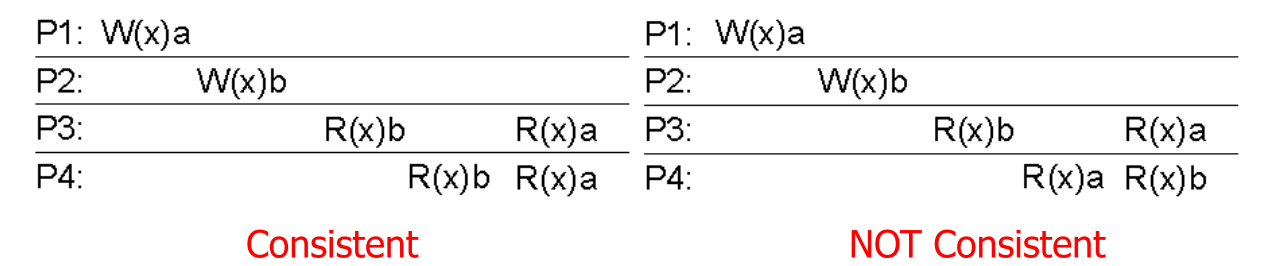
\includegraphics[width=\textwidth]{src/images/consistency-replication/sequential.png}
\caption{An example of sequential consistency}
\end{figure}

\emph{Note that:} for some reasons, we don't care which, the sequential
order here is \emph{b -\textgreater{} a}, so the \emph{image1} is
consistent, because either \emph{P3} and \emph{P4} read the value
\emph{x} in the same order. This is not true in the \emph{image2} and
this is contradictory.

\subparagraph{Why use sequential
consistency?}\label{why-use-sequential-consistency}

This is the best practician protocol to apply also to parallel systems
\emph{(e.g.~DBMS or shared memory on multi-prcocessor computers)}.

\subparagraph{\emph{Java example}}\label{java-example}

Java doesn't use sequential consistency because it's a distributed
system, in the sense of it doesn't share memory, like a parallel system.
This is true because of the cost of implementing a sequential
consistency. In fact it's necessary that all processes agree on a shared
order, and this is expensive.

In practice programming languages implement sequential consistency only
when is needed, that is when the variable is declared as \emph{volatile}
or there is a \emph{synchronized block}.\\
\paragraph{Implementation}

\begin{itemize}
    \item
      All replicas need to agree on a given order of operations, so we need
      a \textbf{single leader} or a \textbf{distributed agreement}.
    \item
      The data sent is \textbf{semi-synchronous}
      
    \item
      Sequential consistency limits availability
    \begin{itemize}
        \item
          We need to contact the leader, \emph{that might be further away from
          the client}
        \item
          The leader must propagate the update to the replicas, \emph{in a
          synchronous way if we want to be fault tolerance}
        \item
          This causes us some problems, such as \emph{high latency}
        \item
          Clients are blocked in the case of network partitions, because it can
          only proceed if they can contact the leader, and this can only proceed
          if it can contact followers
    \end{itemize}
\end{itemize}

\subparagraph{Assumption}
Sticky clients, in the sense of they access always to the same
replica. This is not so useful, because they already agree on the
order.

\subsubsection{Leaderless protocols}

\textbf{Idea} An update occurs only if a quorum of the servers agrees on
the version number to be assigned.
Moreover, reading requires a quorum to ensure latest version is being
read.
We define:
\begin{itemize}
    \item
      $N$: number of total nodes
    \item
      $NR$: number of nodes reading
    \item
      $NW$: number of nodes writing
\end{itemize}
We need that those two condition are satisfied:
\begin{itemize}
    \item
      $NR + NW \gt N$
    \item
      $NW \gt N/2$
\end{itemize}

\textbf{Note that}, in these conditions we are sure that, even in the worst case, there is
always an overlapping on \emph{R} and \emph{W}.

There is also an extreme approach that anyway satisfy the above
conditions, and it's called \textbf{\emph{ROWA (read one, write all)}},
and this is the opposite of the single leader approach.

\begin{figure}[htbp]
    \centering
    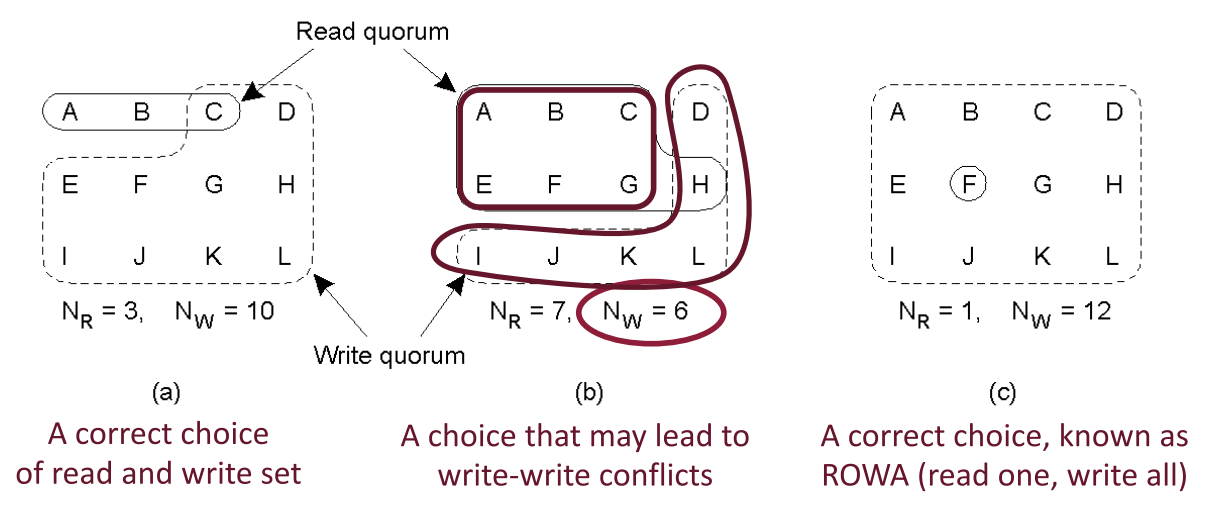
\includegraphics[width=\textwidth]{src/images/consistency-replication/rowa.png}
    \caption{The ROWA procedure}
\end{figure}

\subsubsection{Linearizability}

\textbf{Def.} The system is sequentially consistent; moreover, if
\emph{tsOP1(x) \textless{} tsOP2(y)} then the operation \emph{OP1(x)}
precedes \emph{OP2(y)} in the operation sequence.\\
\textbf{Idea} There is a sequence and we impose it's based on timestamp.\\
\textbf{Assumptions} We must have globally available clocks but only with finite precision.

\subsubsection{Causal consistency}

\textbf{Def.} Writes that are potentially causally related must be seen
by all processes in the same order. Concurrent writes may be seen in any
order at different machines.\\
\textbf{Idea} I understand the meaning of a group of message because of
their order.\\
\textbf{Note that}, it's the same principle on that I can understand the meaning of a
message because I read another message before \emph{(e.g.~in a chat)}.

It's important to notice that I don't want to have a specific sequence for everything, but,
if there are any messages with some kind of relationship I have to
obtain some kind of agreement on the sequence, otherwise I can loss the
relationship and not full understand the semantic.\\
\\
\textbf{Some definitions}

\textbf{Causal order}: a write operation W by a process P is causally
ordered after every previous operation O by the same process, even if W
and O are performed on different variables.

\textbf{Concurrent:} operations that are not causally ordered are said
to be concurrent\\
\\
\textbf{Implementation}\\
Writes are timestamped with Lamport's vector
clock and this implementation enabled a high degree of availability.
This is the same principle I apply when a reply on WhatsApp and I'm
offline. I can replay to messages which I see at the moment.

When I'm offline and I write the rest of the world will not be informed,
so the writes that occur in the rest of the world will be concurrent.

\subsubsection{FIFO consistency}

\textbf{Def.} Writes done by a single process are seen by all others in
the order in which they were issued; writes from different processes may
be seen in any order at different machines.

\textbf{Idea} I have to check only the writes of the same process which
must be read in the same order

\begin{center}\rule{3in}{0.4pt}\end{center}

\subsection{Synchronized models}

Writes become visible only when processes explicitly request so through
the variable, providing appropriate constructs. In practice, it's up to
the programmer to force consistency when needed.

\subsubsection{Weak consistency}

\textbf{Procedure}
\begin{enumerate}
    \def\labelenumi{\arabic{enumi}.}
    \itemsep1pt\parskip0pt\parsep0pt
    \item
      Access to synchronization variables is sequentially consistent
    \item
      No operation on a synchronization variable is allowed until all
      previous writes have completed everywhere
    \item
      No read or write to data are allowed until all previous operations to
      synchronization variables have completed
\end{enumerate}

\begin{figure}[htbp]
    \centering
    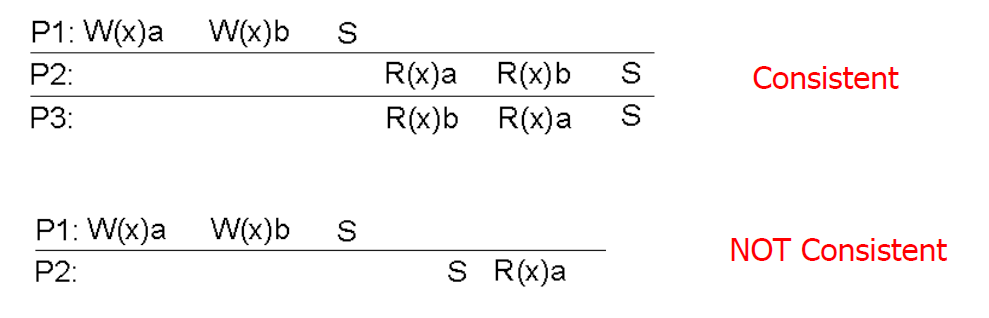
\includegraphics[width=\textwidth]{src/images/consistency-replication/weak-consistency.png}
    \caption{An example of weak consistency implementation}
\end{figure}

\subsubsection{Release consistency}

The previous consistency model has a problem: the data store cannot distinguish between a
synchronization request for disseminating writes or for reading consistent data. A solution is
to introduce different synchronization operations.

\begin{itemize}
    \itemsep1pt\parskip0pt\parsep0pt
    \item
      \emph{Acquire}
    \item
      \emph{Release}
\end{itemize}

\textbf{Procedure}

\begin{enumerate}
    \def\labelenumi{\arabic{enumi}.}
    \itemsep1pt\parskip0pt\parsep0pt
    \item
      Before a read or write is performed, all previous acquires done by the
      process must have completed successfully
    \item
      Before a release is allowed, all previous reads and writes done by the
      process must have been completed
    \item
      Accesses to synchronization variables are FIFO consistent
\end{enumerate}
Two ways to achieve updates:

\begin{itemize}
    \itemsep1pt\parskip0pt\parsep0pt
    \item
      \emph{Eager release}: on release all updates are pushed to other
      replicas
    \item
      \emph{Lazy release}: on acquire, acquiring process must get latest
      version from the data from other processes
\end{itemize}

\subsubsection{Entry consistency}

\textbf{Idea} Explicitly associates each shared data item with a
synchronization variable.\\
Two ways of access to a synchronized variable

\begin{itemize}
    \itemsep1pt\parskip0pt\parsep0pt
    \item
      \emph{Non-exclusive}: multiple processes can hold read locks
      simultaneously
    \item
      \emph{Exclusive}: only one process holds the lock to the variable
\end{itemize}

\textbf{Procedure}

\begin{enumerate}
    \def\labelenumi{\arabic{enumi}.}
    \itemsep1pt\parskip0pt\parsep0pt
    \item
      An acquire access of a synchronization variable is not allowed to
      perform w.r.t. a process until all updates to the guarded shared data
      have been performed w.r.t. that process
    \item
      Before an exclusive mode access to a synchronization variable by a
      process is allowed to perform w.r.t. that process, no other process may
      hold the synchronization variable, not even in non-exclusive mode
    \item
      After an exclusive mode access to a synchronization variable has been
      performed, any other process' next non-exclusive mode access to that
      synchronization variable may not be performed until it has performed
      w.r.t. to that variable's owner
\end{enumerate}

\begin{figure}[htbp]
    \centering
    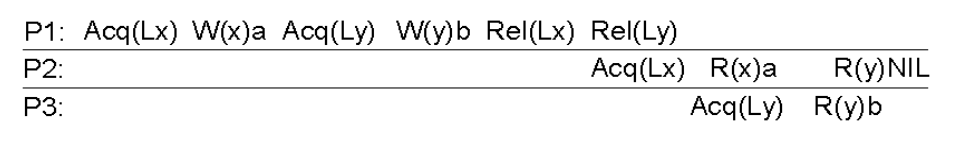
\includegraphics{src/images/consistency-replication/entry-consistency.png}
    \caption{An example of entry consistency implementation}
\end{figure}

\subsection{Summary of consistency models}

\begin{figure}[htbp]
    \centering
    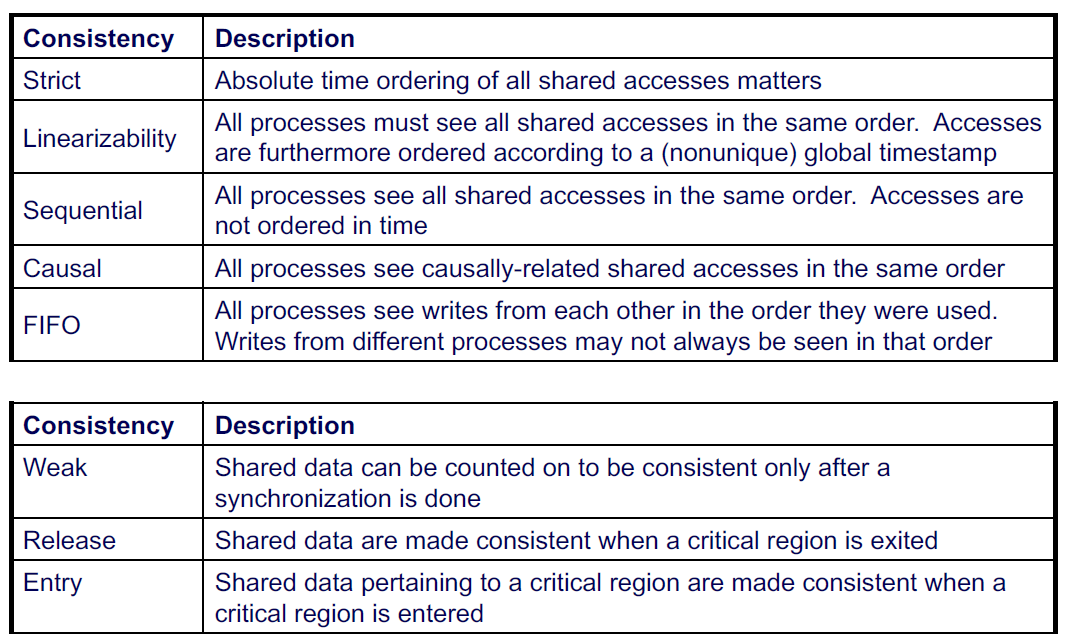
\includegraphics{src/images/consistency-replication/summary.png}
    \caption{Summary of consistency models previously seen}
\end{figure}

\begin{center}\rule{3in}{0.4pt}\end{center}

\paragraph{Eventual consistency}

\textbf{Idea} Eventually, you will receive updates

\emph{Intro:} there are situations in which there are no simultaneous
updates, or can easily resolved (\emph{e.g.~highest ID wins}) and mostly
reads

In practice, this system is often sufficient: updates are guaranteed to
eventually propagate to all replicas.

\textbf{Conflict-free replicated data types} guarantee convergence even
if updates are received in different orders. In this case we guarantee
the convergence of the result (\emph{e.g.~integer counter})

\begin{center}\rule{3in}{0.4pt}\end{center}

\subsubsection{Client-centric
consistency}\label{client-centric-consistency}

\emph{Problem:} What happens if a client dynamically changes the replica
it connects to?

\paragraph{Monotonic reads}\label{monotonic-reads}

\textbf{Def.} If a process reads the value of a data item \emph{x}, any
successive read operation on \emph{x} by that process will always return
that same value or a more recent value

\textbf{Idea} Once a process reads a value from a replica, it will never
see an older value from a read at a different replica

\begin{figure}[htbp]
\centering
\includegraphics{C:/Users/Davide/AppData/Roaming/Typora/typora-user-images/image-20200103163647355.png}
\caption{image-20200103163647355}
\end{figure}

\paragraph{Monotonic writes}\label{monotonic-writes}

\textbf{Def.} A write operation by a process on a data item \emph{x} is
completed before any successive write operation on \emph{x} by the same
process.

It's similar to \emph{FIFO consistency}, although this time for a single
process

\begin{figure}[htbp]
\centering
\includegraphics{C:/Users/Davide/AppData/Roaming/Typora/typora-user-images/image-20200103172406404.png}
\caption{image-20200103172406404}
\end{figure}

\paragraph{Read your writes}\label{read-your-writes}

\textbf{Def.} The effect of a write operation by a process on a data
item \emph{x} will always be seen by a successive read operation on
\emph{x} by the same process

\begin{figure}[htbp]
\centering
\includegraphics{C:/Users/Davide/AppData/Roaming/Typora/typora-user-images/image-20200103172527259.png}
\caption{image-20200103172527259}
\end{figure}

\paragraph{Writes follow reads}\label{writes-follow-reads}

\textbf{Def.} A write operation by a process on a data item \emph{x}
following a previous read operation on \emph{x} by the same process is
guaranteed to take place on the same or more recent value of \emph{x}
that was read

\begin{figure}[htbp]
\centering
\includegraphics{C:/Users/Davide/AppData/Roaming/Typora/typora-user-images/image-20200103172733976.png}
\caption{image-20200103172733976}
\end{figure}

\paragraph{Implementation}\label{implementation-1}

\begin{itemize}
\itemsep1pt\parskip0pt\parsep0pt
\item
  Each operation gets a unique identifier
\item
  Two sets are defined for each client
\item
  Read-set: the write identifiers relevant for the read operations
  performed by the client
\item
  Write-set: the identifiers of the write performed by the client
\item
  It can be encoded as vector clocks
\end{itemize}

\begin{center}\rule{3in}{0.4pt}\end{center}

\subsection{Design strategies}\label{design-strategies}

\subsubsection{Replica placement}\label{replica-placement}

\begin{itemize}
\itemsep1pt\parskip0pt\parsep0pt
\item
  Permanent replicas: statically configured
\item
  Server-initiated replicas:
\item
  Create dynamically
\item
  Move data closer to clients
\item
  Often require topological knowledge
\item
  Client-initiated replicas: rely on a client cache
\end{itemize}

\begin{figure}[htbp]
\centering
\includegraphics{C:/Users/Davide/AppData/Roaming/Typora/typora-user-images/image-20200103173810593.png}
\caption{image-20200103173810593}
\end{figure}

\subsubsection{Update propagation}\label{update-propagation}

\begin{itemize}
\itemsep1pt\parskip0pt\parsep0pt
\item
  Perform the update and propagate only a notification (works best if
  \emph{\#reads \textless{}\textless{} \#writes})
\item
  Transfer the modified data to all copies (works best if \emph{\#reads
  \textgreater{}\textgreater{} \#writes})
\item
  Propagate information to enable the update operation to occur at other
  copies (we need to take into account side effects)
\end{itemize}

\paragraph{How do this?}\label{how-do-this}

\begin{itemize}
\itemsep1pt\parskip0pt\parsep0pt
\item
  Push-based approach: the update is propagated to all replicas,
  regardless of their needs
\item
  Pull-based approach: an update is fetched on demand when needed and
  this is more convenient if \emph{\#reads \textless{}\textless{}
  \#writes}
\end{itemize}

\paragraph{Propagation strategies}\label{propagation-strategies}

\begin{itemize}
\itemsep1pt\parskip0pt\parsep0pt
\item
  Anti-entropy: server chooses another at random and exchanges updates
\item
  Gossiping: an update propagation triggers another towards a different
  server, and the server reduces the probability to gossip further as
  the updates arrives continuously
\item
  Intrinsically distributed, redundant, scalable, fault-tolerant and
  resilient to topological changes
\end{itemize}

\begin{center}\rule{3in}{0.4pt}\end{center}

\subsubsection{Transactional models}\label{transactional-models}

Data consistency is a key aspect in distributed databases.

Transactions define groups of operations and provide ACID guarantees
atomicity, consistency, isolation and durability.
